\chapter{Infrastructure Management Planning}\label{ch:impmarl}

\begin{chapter_outline}

This chapter presents IMP-MARL, an open-source suite of multi-agent reinforcement learning environments for large-scale infrastructure management planning.
In section \ref{sec:ch5_intro}, we introduce the problem behind infrastructure management planning and the motivations behind it.

and the contributions of this chapter, followed the history behind this application in section \ref{sec:ch5_relatedwork}.

This chapter is an adapted version of the publication \citep{leroy2023impmarl} \textit{IMP-MARL: a suite of environments for large-scale infrastructure management planning via MARL}, P. Leroy, P. G. Morato, J. Pisane, A. Kolios, and D. Ernst. Thirty-seventh Conference on Neural Information Processing Systems Datasets and Benchmarks Track, 2023.
\end{chapter_outline}

\section{Introduction}\label{sec:ch5_intro}
Multiple suite of environments based on games and simulators have served as benchmark testbeds to support the advancement of cooperative MARL methods and are presented in Section \ref{sec:ch3_env}.
Benchmarking environments based on games and simulators is useful for the development of MARL methods in specific collaborative/competitive tasks.
However, additional challenges may still be encountered when deploying MARL methods in real-world applications \citep{oroojlooy2022review}.

Infrastructure Management Planning (IMP) is a contemporary application that responds to current societal and environmental concerns.
In IMP, inspections, repairs, and/or retrofits should be timely planned to control the risk of potential system failures, e.g., bridge and wind turbine failures, among many others \citep{morato2022optimal}.
The system failure risk is defined as the system failure probability multiplied by the consequences associated with a failure event, typically defined in monetary units.
Due to model and measurement uncertainties, the components' damage is not perfectly known, and decisions are made based on a probability distribution over the damage condition, henceforth denoted as damage probability.
The system failure probability is a function of components' damage probabilities.
Starting from its initial damage distribution, each component's damage probability transitions according to a deterioration stochastic process and to the decisions made~\citep{morato2022optimal}.
Naturally, the damage probability transitions based on its deterioration model when the component is neither inspected nor repaired, i.e., do-nothing action.
If a component is inspected, its damage probability is updated based on the inspection outcome.
When a component is repaired, its damage condition is directly improved, and the damage probability resets to its initial damage distribution.
A schematic of a typical IMP problem is shown in Figure \ref{fig:ch5_imp_problem}.

\begin{figure}
\centering
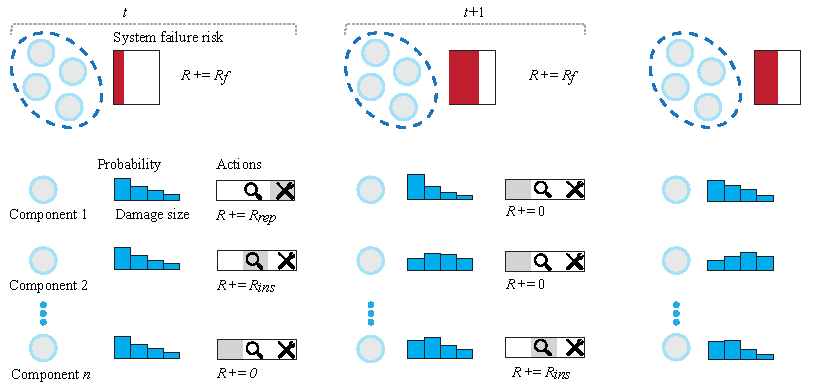
\includegraphics[width=\textwidth]{tex_thesis/figures/ch5/imp_intro.pdf}
\caption{Overarching representation of an infrastructure management planning (IMP) problem.
The system failure risk is defined as a function of the probability distribution over the components' damage condition. 
To control the system failure risk, components can be inspected or repaired at each time step $t$ and, typically, an agent controls one component.
The objective of IMP's problem is the maximisation of the expected sum of discounted rewards, by balancing the system failure risk $R_f$ against inspections $R_{ins}$ and repairs $R_{rep}$, all three being negative rewards.
Here, we show three components with the same damage probability at time step $t$.
When a component is not inspected nor repaired, its damage probability evolves according to a deterioration process. If a component is inspected, information from the inspection is also considered when updating the damage probability, and if a component is repaired, the damage probability resets to its initial damage distribution.}
\label{fig:ch5_imp_problem}
\end{figure}

IMP-MARL was introduced to generate more efficient strategies for managing engineering systems through cooperative MARL methods.
In IMP-MARL, each agent is responsible for managing one constituent component in a system, making decisions based on the damage probability of the component.
Besides seeking to reduce component inspection and maintenance costs, agents should effectively cooperate to minimise the system failure risk.

With IMP-MARL, an additional goal is to facilitate the definition and implementation of new customisable environments.
Moreover, by jointly minimising system failure risks and inspection/maintenance costs, more effective IMP policies contribute to a better allocation of resources from a societal perspective.
Additional societal impact is also made by controlling the risk of system failure events.
For example, the failure of a wind turbine may affect the available electricity production. 
Beyond economic considerations, our proposed IMP-MARL framework can also be used to include sustainability and societal metrics within the objective function by accounting for those directly in the reward model.

To assess the capability of cooperative MARL methods for generating effective policies for IMP problems involving many components, we additionally benchmark here state-of-the-art cooperative MARL methods in terms of scalability and optimality.
The benchmarked methods are presented in Chapter \ref{part:background} and Chapter \ref{ch:cooperation}.
Specifically, we benchmark five CTDE methods: QMIX, QVMix, QPLEX, COMA, and FACMAC, along with a decentralised method, i.e., IQL, and a centralised one, i.e., DQN.
All tested MARL methods are compared against expert-based heuristic policies, which can be categorised as a state-of-the-art method to deal with IMP problems in the reliability engineering community \citep{LuqueDBN2019, morato2022optimal}.
In our study, three sets of IMP environments are investigated, including one related to offshore wind structural systems, where MARL methods are tested with up to 100 agents.
Additionally, these environments can be set up with two distinct reward models, and one of them incorporates explicit cooperative objectives.
For the sake of enabling the reproduction of any published result, we have made our best effort to ensure that the necessary code is publicly available.

Finally, the contributions of \citep{leroy2023impmarl} presented in this chapter can be outlined as follows:
\begin{itemize}
  \item IMP-MARL is an open-source suite of environments, motivating the development of scalable MARL methods as well as the creation of new IMP environments, enabling the effective management of multi-component engineering systems and, as such, leading to a positive societal impact.
  \item In an extensive benchmark campaign, we test state-of-the-art cooperative MARL methods in very high-dimensional IMP environments featuring up to 100 agents.
  The resulting management strategies are evaluated against expert-based heuristic policies.
  We publicly provide the source code for reproducing our reported results and for easing direct comparisons with future developments.
  \item Based on our results, we draw relevant insights for both machine learning and reliability engineering communities, further highlighting important challenges that must still be resolved.
  While cooperative MARL methods can learn superior strategies compared to expert-based heuristic policies, the relative performance benefit decreases in environments with over 50 agents.
  In certain environments, cooperative MARL policies are characterised by a high variance and sometimes underperform expert-based heuristic policies, suggesting the need for further research efforts.
\end{itemize}

\todo{jointly observable oliehoek, agenti-wise factored dec-pomdp}
\todo{multi agent mdp}


\section{Related work} \label{sec:ch5_relatedwork}
Recent heuristic-based inspection and maintenance (I\&M) planning methods generate IMP policies based on an optimised set of predefined decision rules \citep{LuqueDBN2019, Bismut2019OptimalDete}.
By evaluating only a set of decision rules out of the entire policy space, the previously mentioned approaches might yield suboptimal policies \citep{morato2022optimal}.
In the literature, one can also find POMDP-based methods applied to the I\&M planning of engineering components, in most cases, relying on efficient point-based solvers \citep{Papakonstantinou2014Part1, Papakonstantinou2014Part2, morato2022optimal}. 
When dealing with multi-component engineering systems, solving point-based POMDPs becomes computationally complex.
In that case, the policy and value function can be approximated by neural networks, enabling the treatment of high-dimensional engineering systems.
Specifically, actor-critic, and value function-based methods have been proposed in the literature for the management of engineering systems \citep{Andriotis2019ManagingLearning,andriotis2021deep,morato2022syst} with some of them relying on CTDE methods \citep{nguyen2022weighted, saifullah2022deep}. Note that no open-source methods nor publicly available environments are provided in the above-mentioned references.
This emphasises the importance of our efforts to enhance comparison and reproducibility within the reliability engineering community.


\section{IMP-MARL: A suite of Infrastructure Management Planning environments} \label{sec:ch5_imp}

In IMP, the damage condition of multiple components deteriorates stochastically over time, inducing a system failure risk that is penalised at each time step.
To control the system failure risk, components can be inspected or repaired, yet, incurring additional costs.
The objective is the minimisation of the expected sum of discounted costs, including inspections, repairs, and system failure risk.
This can be achieved through the agents' cooperative behaviour, assigning component inspections and repairs while jointly controlling the system failure risk.
The introduced IMP decision-making problem can be modelled as a decentralised partially observable Markov decision process (Dec-POMDP).

\subsection{Environments formulation}
\label{sec:env_formulation}
\textbf{States and observations}
As introduced, each agent in IMP perceives $o^a_t$, an observation corresponding to its respective component damage probability and the current time step.
Each component damage probability transitions based on a deterioration model, defined according to physics-based engineering models, e.g., numerical simulators and/or analytical laws~\citep{Papakonstantinou2014Part1}.
The damage probability is also updated based on maintenance decisions.
Since the components' damage is not perfectly known, the state of the Dec-POMDP is defined as the collection of all components' damage probabilities along with the current time step: $s_t = (o_t^1, .., o_t^n, t)$.
This is called a jointly observable Dec-POMDP that is also referred to as a decentralised MDP in \citep{DecPomdp}.
However, this does not make the problem simpler because each agent still does not observe this state \citep{bernstein2002complexity}.
\todo{check if we do not want to address this in chapter 3.}


\textbf{Actions and rewards}
Each agent controls a component and collaborates with other agents in order to minimise the system failure risk while minimising local costs associated with individual repair and/or inspection actions. 
At each time step $t$, an agent decides $u^a_t$ between (i) do-nothing, (ii) inspect, or (iii) repair actions.
Both inspection and repair actions incur significant costs, formally included in the Dec-POMDP framework as negative rewards, $R_{ins}$ and $R_{rep}$, respectively.
Moreover, the system failure risk is defined as $R_f= c_F \cdot p_{F_{sys}}$ where $p_{F_{sys}}$ is the system failure probability and $c_F$ is the associated consequences of a failure event, encompassing economic, environmental, and societal losses.
In IMP, we include two reward models.
The first is a \emph{campaign cost} model where a global cost, $R_{camp}$, is incurred if at least one component is inspected or repaired, plus a surplus, $R_{ins}$ + $R_{rep}$, per inspected/repaired component.
This campaign cost explicitly incentivises agents to cooperate.
The second is a \emph{no campaign cost} model, where the campaign cost is set equal to 0 (i.e., $R_{camp}=0$), and only component inspections and repairs costs are considered. 
Acting on finite-horizon episodes that span over $T$ time steps, all agents aim at maximising the expected sum of discounted rewards $\mathbb{E}[R_{0}] = \mathbb{E} \left[ \sum_{t=0}^{T-1} \gamma^t \left[ R_{t,f}+ \sum_{a=1}^n \left({R_{t,ins}^a} + {R_{t,rep}^a}\right)+R_{t,camp} \right] \right]$.

\textbf{Real-world data} While IMP policies are trained based on simulated data, they policies can then be deployed to applications where real-world streams of data are available. In that case, the damage condition of the components is updated based on collected real-world data, e.g., inspections.
 
\subsection{IMP-MARL environments}
\label{time stepsec:implement_env}

With IMP-MARL, we provide three sets of environments to benchmark cooperative MARL methods.
For all three, components are exposed to fatigue deterioration during a finite-horizon episode, inducing the growth of a crack over $T$ time steps.
The first set of environments is named \textit{k-out-of-n system} and refers to systems for which a system failure occurs if (n-k+1) components fail.
Those systems have been widely studied in the reliability engineering community~\citep{barlow1984computing}. 
The second type of generic environment is named \textit{correlated k-out-of-n system} and is a variation of the first one for which the initial components' damage distributions are correlated.
The last one is named \textit{offshore wind farm} and allows the definition of environments for which a group of offshore wind turbines must be maintained.
The proposed IMP-MARL environment sets and options are graphically illustrated in Figure \ref{fig:env_categories}, and we hereafter provide details about these sets of environments.
Additionally, the deterioration processes and implementation details are formally described in the following Section \ref{App:pomdpModels} and Section \ref{App:envir}.

\textbf{k-out-of-n system}
In this set of environments, the components' damage probability distribution, $p(d^a_t)$, is defined as a vector of 30 bins, with each bin representing a crack size interval.
Here, the failure probability of one component is defined as the probability indicated in the last bin.
The specificity of a k-out-of-n system is that it fails if (n-k+1) components fail, establishing a direct link between the system failure probability and the component failure probabilities.
For this first system, the initial damage distribution is statistically independent among components and the time horizon is $T=30$ time steps.
Since it is finite, we normalise each time step input and we define $s_t = (p(d^1_t),..., p(d^n_t), t/T)$ and $o^a_t=(p(d^a_t), t/T)$.
The interest of this system is that, in many practical scenarios, the reliability of an engineering system can be modelled as a \textit{k-out-of-n system}.

\textbf{Correlated k-out-of-n system}
The second set of environments is the same as the first one previously defined, with the difference that the initial damage distribution is correlated among all components.
Therefore, inspecting one component also provides information about other uninspected components, depending on the specified degree of correlation.
This setting is particularly challenging when approached from a decentralised scheme without providing components' correlation information to individual agents.
To further address this issue, and in addition to their 30-bin local damage probability, the agents perceive correlation information $\alpha_t$ common to all, which is updated based on inspection outcomes collected from all components.
We thus have: $s_t = (p(d^1_t),..., p(d^n_t),\alpha_t, t/T)$ and $o^a_t=(p(d^a_t), \alpha_t, t/T)$.
This damage correlation structure is inspired by practical engineering applications where initial defects among components are statistically correlated due to the fact that components undergo similar manufacturing processes \citep{morato2022optimal}.

\textbf{Offshore wind farm}
The third set of environments is different from the previous ones as it considers a system with a certain number of wind turbines.
Specifically, each wind turbine contains three representative components: (i) the top component located in the atmospheric zone, (ii) the middle component in the underwater zone, and (iii) the mudline component submerged under the seabed.
In this case, we consider that the mudline component cannot be inspected nor repaired, as it is installed under the seabed in an inaccessible region and, since only the top and middle components can be inspected or repaired, two agents are assigned for each wind turbine.
Furthermore, the damage probability, $p(d^a_t)$, is a vector with 60 bins and transitions differently depending on the component location in the wind turbine, as corrosion-induced effects accelerate deterioration in certain areas. 
Besides individual component damage models, inspection techniques and their associated costs also depend on the component location: it is cheaper to inspect or repair the top components than the middle one \citep{giro2022inspection}.
Moreover, while the mudline component cannot be directly maintained, its damage probability also impacts the failure risk of a wind turbine.
In offshore wind farm environments, a wind turbine fails if any of its three constituent components fails, and the overall system failure risk is defined as the sum of all individual wind turbine failure risks. In this case, $p(d^a_t)$ is modelled as a 60-bin vector and the time horizon is $T=20$.
In this set of environments $s_t = (p(d^1_t),..., p(d^n_t), t/T)$ and $o^a_t=(p(d^a_t), t/T)$.

\begin{figure}
\begin{subfigure}[t]{0.53\textwidth}
\centering
    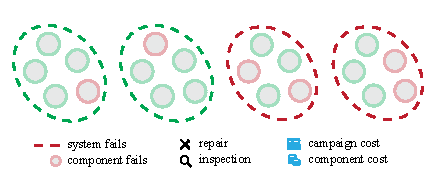
\includegraphics[width=1\linewidth]{tex_thesis/figures/ch5/fig2_mul/environments_v2_a.pdf}
    \caption{A k-out-of-n system environment.}
    \label{fig:env_categories_1}
\end{subfigure}%
\begin{subfigure}[t]{0.47\textwidth}
\centering
    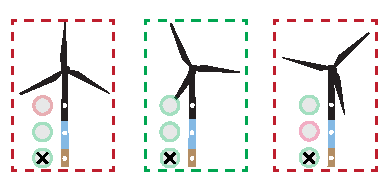
\includegraphics[width=1\linewidth]{tex_thesis/figures/ch5/fig2_mul/environments_v2_b.pdf}
    \caption{An offshore wind farm environment.}
    \label{fig:env_categories_2}
\end{subfigure}
%
\begin{subfigure}[t]{0.53\textwidth}
\centering
    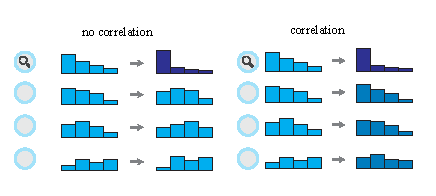
\includegraphics[width=1\linewidth]{tex_thesis/figures/ch5/fig2_mul/environments_v2_c.pdf}
    \caption{Uncorrelated and correlated initial damage distribution.}
    \label{fig:env_categories_3}
\end{subfigure}%
\begin{subfigure}[t]{0.47\textwidth}
\centering
    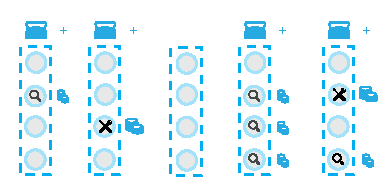
\includegraphics[width=1\linewidth]{tex_thesis/figures/ch5/fig2_mul/environments_v2_d.pdf}
    \caption{A campaign cost environment.}
    \label{fig:env_categories_4}
\end{subfigure}
\caption{
Visual representation of available IMP-MARL environment sets and options.
In \ref{fig:env_categories_1}, a 4-out-of-5 system fails if 2 or more components fail.
In \ref{fig:env_categories_2}, a wind turbine fails if any constituent component fails.
In \ref{fig:env_categories_3}, when the environment is under deterioration correlation, the information collected by inspecting one component also influences uninspected components.
In \ref{fig:env_categories_4} campaign cost environments, a global cost is incurred if any component is inspected and/or repaired plus a surplus per inspected/repaired component. 
}
\label{fig:env_categories}
\end{figure}



\section{Modelling infrastructure management in IMP-MARL}
\label{App:pomdpModels}
In this section, we thoroughly describe the deterioration, inspection, and transition models implemented in this work. 
These models drive the dynamics of the IMP-MARL environments provided in this paper.
Based on this information, one can easily learn how to create new environments.

\subsection{Deterioration models}
The deterioration processes introduced here specifically correspond to fatigue deterioration mechanisms, yet corrosion, erosion, and many other practical infrastructure management problems can be similarly modelled.

\textbf{Correlated and uncorrelated k-out-of-n systems}
Throughout the text and the code, the set of environments related to correlated and uncorrelated k-out-of-n systems are abbreviated as struct\_c and struct\_uc, respectively, or denoted as struct when referring to both of them. 
In the k-out-of-n environments currently included in IMP-MARL, the structural components are exposed to fatigue deterioration, and unless a repair is undertaken, the crack size $d_t$  (i.e., damage condition) evolves over time $t$ as \citep{Ditlevsen2007StructuralMethods}: 
\begin{equation} \label{Eq:ExamCrackGrow}
d_{t+1} =\bigg[ \Big(1-\frac{m}{2}\Big) C_{FM}S_{R}^m\pi ^{m/2}n_{S} + d_t^{1-m/2}\bigg] ^{2/(2-m)} \, ,
\end{equation}
where $\ln(C_{FM}) \sim \mathcal{N} (\mu=-35.2, \sigma=0.5)$ and $m=3.5$ stand for material variables, which directly influence the crack growth.
Due to environmental and operational conditions, the components are subject to a dynamic load characterised by the stress range, $S_{R}  \sim  \mathcal{N} (\mu=70, \sigma=10$ N/mm$^2$), over $n_{S}=10^6$ annual stress cycles, i.e., the number of load cycles experienced by the structural component in one year.
At the initial step or after a component is repaired, the initial crack size is at its intact condition, defined by its initial distribution $d_0  \sim  \text{Exp} (\mu=1$ mm), and a component level failure occurs when the crack size exceeds a critical size of $d_c=20$ mm. 
The component failure probability $p_{F}$, defined as $p_{F}=p[g \leq 0]$, can be computed following a through-thickness failure criterion \cite{hlaing2022inspection}, where the failure limit at time step $t$ is formulated as $g_{t}=d_c-d_t$. At the system level, a failure event occurs if $k$ (out of $n$) components fail, and its corresponding system failure probability, $p_{F_{sys}}$, can be efficiently computed as a function of all components failure probabilities, as proposed in \citep{barlow1984computing}. 

The continuous crack size is discretised into a certain number of discrete bins in order to enable efficient Bayesian inference once inspection indications are available.
Further details can be found in \citep{morato2022optimal}. 
If the initial crack size among components is correlated (i.e., we are dealing with a correlated k-out-of-n system), the damage condition of each component is defined conditional on a common correlation factor, $\alpha$, via a Gaussian hierarchical structure \citep{morato2022syst}.
In that case, the discretised damage bins should be defined conditional on the correlation factor.
The specific discretisation implemented in our environments is defined in Table \ref{Tab:discrExam}. 

\begin{table}
\caption{Description of the discretisation scheme implemented.}\label{Tab:discrExam}
\begin{tabular}{llll}
\toprule
Environment & Variable & Interval boundaries & Bins\\
\midrule
struct & $d_t$ & $[0, \mathrm{exp}\{ \mathrm{ln}(10^{-4}):(\mathrm{ln}(d_{c})-\mathrm{ln}(10^{-4}))/28:\mathrm{ln}(d_{c})\},\infty ]$ & 30 \\
owf & $d_t$ & $[0, d_0:(d_c-d_0)/(60-2):d_c,\infty]$ & 60 \\
\bottomrule
\end{tabular}
\end{table}

\textbf{Offshore wind farm}
In this set of environments, a group of \texttt{n\_comp} offshore wind substructures is considered, in which three representative structural components are modelled at different locations of the wind turbine: (i) at the atmospheric zone - upper level, (ii) at the splash zone - middle level, (iii) below the seabed - mudline. 
The deterioration, inspection, and cost models hence differ for each of the three considered components. While the fatigue deterioration is calculated according to Eq. \ref{Eq:ExamCrackGrow}, the expected dynamic load, $S_r$, is in this case defined based on industrial standards \citep{dnv2015probabilistic}, as: 
\begin{equation}
    S_r = q\Gamma(1+1/\lambda)Y \, ,
    \label{eq:ex_eqstr}
\end{equation}
corresponding to the expected value of a Weibull distribution defined by the scale parameters listed in Table \ref{tab:owf_fatigue}, $q \sim \mathcal{N}$, and shape factor, $\lambda=0.8$, weighted by a geometric parameter, $Y  \sim  \mathcal{LN} (\mu=0.1, \sigma=0.1)$. The initial crack size distribution is specified for all wind turbine components as $d_0  \sim  \text{Exp} (\mu=0.11)$ and the remaining specific fatigue variables associated with each wind turbine component are listed in Table \ref{tab:owf_fatigue}. 
At the wind turbine level, the failure event occurs if one component of the wind turbine fails. 
The wind turbine failure risk is then defined as the wind turbine failure probability multiplied by the consequences associated with a wind turbine failure event.
At the wind farm level, the damage condition of a wind turbine does not influence the condition of the other wind turbines, and the wind farm system failure risk is defined as the sum of all turbines' failure risk.

\begin{table}
\centering
\caption{Variables specified in the offshore wind farm deterioration models.}
\label{tab:owf_fatigue}
\begin{tabular}{lccc}
\toprule
 & Upper component & Middle component & Mudline component  \\
 \midrule
\multirow{2}{*}{$ln(C_{FM})$} & $\mu=-26.45$ & $\mu=-26.04$ & $\mu=-26.12$ \\
& $\sigma=0.12$ & $\sigma=0.4$ &  $\sigma=0.39$ \\
$m$ & 3 & 3 & 3 \\
\multirow{2}{*}{$q$}   & $\mu=10.21$  & $\mu=7.40$ & $\mu=6.74$  \\
 & $CoV=25\% $  & $CoV=25\% $ & $CoV=25\% $  \\
$d_c$ & 20 & 60 & 60 \\
$n_{S}$ & 5,049,216 & 5,049,216 & 5,049,216
\\
\bottomrule
\end{tabular}
\end{table}

\subsection{Inspection models}
The inspection models implemented in IMP-MARL are hereafter described, defining the likelihood of retrieving a certain inspection outcome as a function of the damage size.

\textbf{Correlated and uncorrelated k-out-of-n systems}
The inspection model is normally characterised depending on the accuracy of the measurement instrument, formally specified through probability of detection (PoD) curves, in which the probability of observing a crack is defined as a function of the crack size \citep{morato2022optimal}.
In this case, the inspection model is described by an exponential distribution $p({i_{d_t}}|d_t) \sim \text{Exp}(\mu = 8)$, defining the probability of observing a crack during an inspection.

\textbf{Offshore wind farm}
In this more practical set of environments, an eddy current inspection technique is here considered, whose PoD can be modelled according to industrial standards \citep{dnv2015probabilistic}, as:
\begin{equation} \label{eq:ex_pod1}
    p({i_{d_t}}|d_t) = 1 - \frac{1}{1+(d_t/\chi)^b}, 
\end{equation}
where the factors $\chi$ and $b$ are specified as 0.4 and 1.43, respectively, for the upper component, but considered as 1.16 and 0.90, for the middle component.
Naturally, less accurate inspection outcomes can be expected for the middle component, as it is located in a region below the water level, where the visibility is reduced.

\subsection{Transition models}
An overview of the transition model is explained hereafter.
For a more detailed description, we refer the reader to \citep{morato2022syst}.
Since the crack size is discretised in this work, the transition and inspection models can be stored in tables.
In our code, they are encoded in Numpy files, which are stored in the repository folder \texttt{pomdp\_models}.
In particular, the files are named \texttt{Dr3031C10.npz}, \texttt{Dr3031\_H08.npz}, and \texttt{owf6021.npz}, for k-out-of-n system, correlated k-out-of-n system, and offshore wind farm, respectively.
By relying on already stored transition and inspection models, the environments can be simulated efficiently.
Alternatively, the crack size evolution could also be directly computed at execution time, yet an additional computational expense would be then incurred.

The transition model can be defined based on the deterioration and inspection models previously described. 
If no inspection and maintenance are taken (i.e. do-nothing action), the damage condition progresses each time step according to the fatigue deterioration model formulated in Eq. \ref{Eq:ExamCrackGrow}.
Note that in our three sets of environments, a time step represents a year.
Considering that the damage follows a non-stationary deterioration process, the crack size distribution $d_{t+1}$ can be efficiently encoded as a function of the annual deterioration rate, $\tau_{t+1}$, and the crack size at the previous time step $d_{t}$ as $p(d_{t+1}|d_t,\tau_{t+1})$. 
Starting from $\tau_{0}=0$, the deterioration rate increases by one unit every year, unless a component is repaired, in which case the deterioration rate returns to the initial value. 
The deterioration evolution over a time step can be computed as:
\begin{equation} \label{eq:ex_pod2}
    p(d_{t+1}) =  \sum_{\tau_{t+1}} \sum_{d_t} p(d_{t+1}|d_t,\tau_{t+1}) p(d_{t}) p(\tau_{t+1}) \, .
\end{equation}

If an inspection action is planned, a damage indication $i_{d_{t+1}}$ is collected, and the crack size distribution can be updated via Bayes' rule:
\begin{equation} \label{eq:ex_pod3}
    p(d_{t+1}|i_{d_{t+1}}) \propto  p(i_{d_{t+1}}|d_{t+1}) p(d_{t+1}) \, ,
\end{equation}
where the likelihood corresponds to the specific inspection model, described by a probability of detection curve, as mentioned before.
Since the damage probabilities are discrete, the normalisation constant can be straightforwardly computed by simply summing the unnormalised bins \citep{morato2022optimal}.

To enable efficient computation of the deterioration evolution under correlation, a Gaussian hierarchical structure is adopted \citep{morato2022syst}, in which the crack size probability is defined conditional on a common factor, $\alpha$ as $p(d_{t}|\alpha)$. In this work, we consider that the initial damage probabilities are equally correlated among components with a Pearson coefficient equal to 0.8. 

The damage transitions, in this case, are formulated as: 
\begin{equation} \label{eq:ex_pod4}
    p(d_{t+1}|\alpha) =  \sum_{\tau_{t+1}} \sum_{d_t} p(d_{t+1}|d_t,\tau_{t+1}) p(d_{t}|\alpha) p(\tau_{t+1}) \, .
\end{equation}
Once an inspection outcome is available, the common correlation factor is also updated based on the new information, thus influencing all components. The likelihood of collecting one inspection indication given $\alpha$ can be computed as:
\begin{equation}\label{Eq:margHyp}
p(i_{d_{t+1}}|\alpha)=\sum_{d_{t+1}} \Big[p(d_{t+1}|\alpha)\,p(i_{d_{t+1}}|d_{t+1})\Big] \, ,
\end{equation}
and the correlation factor can then be updated:
\begin{equation}\label{Eq:infHyp}
p(\alpha|i_{d_{t+1}}) \propto p(\alpha)p(i_{d_{t+1}}|\alpha) .
\end{equation}
Finally, the marginal damage probabilities are computed as:
\begin{equation}\label{Eq:margBel}
p(d_{t+1}) = \sum_{\alpha} \Big[p(d_{t+1}|\alpha)\, p({\alpha}) \Big] \, .
\end{equation}
 
\subsection{Reward model}
The goal of the agents is to maximise the expected sum of discounted rewards, $\mathbb{E}[R_{0}] = \mathbb{E} \left[ \sum_{t=0}^{T-1} \gamma^t \left[ R_{t,f}+ \sum_{a=1}^n \left({R_{t,ins}^a} + {R_{t,rep}^a}\right)+R_{t,camp} \right] \right]$, as stated in Section \ref{sec:env_formulation}.
The rewards collected at each time step may include inspection $R_{ins}$ and repair $R_{rep}$ costs for all considered components, along with the system failure risk, which is defined as the system failure probability $p_{f_{sys}}$ multiplied by the associated consequences of a failure event $c_f$, formulated as $R_f = p_{f_{sys}} \cdot c_f$. Additionally, a campaign cost $R_{camp}$ may also be included if that option is active.
The discount factor is defined as $\gamma=0.95$ in our experiments and the specific rewards are listed in Table \ref{tab:rewards_det}.

\begin{table}
\centering
\caption{Rewards specified in our experiments.}
\label{tab:rewards_det}
\begin{tabular}{llllll}
\toprule
Component & Campaign cost & $R_{ins}$ & $R_{rep}$ &  $c_f$ & $R_{camp}$ \\
\bottomrule
\multirow{2}{*}{struct} &  False & -1 & -20 & -10,000 & 0  \\ 
& True & -0.2 & -20 & -10,000 & -5   \\
\bottomrule
\multirow{2}{*}{owf upper level} & False & -1 & -10 & -1,000 & 0     \\
& True  & -0.2 & -10 & -1,000 & -5     \\
\multirow{2}{*}{owf middle level} & False & -4 & -30 & -1,000 & 0    \\
& True & -1 & -30 & -1,000 & -5    \\
\bottomrule
\end{tabular}
\end{table}

\subsection{Implementation}

All defined IMP environments are integrated with well-known MARL ecosystems, i.e., Gym \citep{openaigym}, Gymnasium \citep{towers_gymnasium_2023}, PettingZoo \citep{terry2021pettingzoo} and PyMarl \citep{samvelyan2019starcraft}, through wrappers.
The tested MARL methods are adopted from PyMarl's library, but other libraries are also compatible with our wrappers, e.g., RLlib \citep{liang2018rllib}, CleanRL \citep{huang2022cleanrl}, MARLlib \citep{hu2022marllib}, or TorchRL \citep{bou2023torchrl}.
All developments are available on a public GitHub repository, \url{https://github.com/moratodpg/imp\_marl}, featuring an open-source Apache v2 license.
If you want to reproduce these, the options are given in Appendix 
\section{Experiments}\label{sec:ch5_appendix_imp_public_repo}

\subsection{Tested methods}
\label{sec:tested_method}
In an extensive benchmark campaign, we test seven RL methods.
The centralised controller, which has an action space that scales exponentially with the number of agents, is trained with the fully centralised method DQN and is the only method taking $s_t$ as input.
Furthermore, the fully decentralised method we test is IQL, in which all agents are independently trained.
Regarding the five CTDE methods, we investigate the three value-based methods: QMIX, QVMix, and QPLEX and two actor-critic methods: COMA and FACMAC.
We selected these methods for our benchmark study because they are well established and their implementations are open-sourced and available within the PyMarl framework \citep{samvelyan2019starcraft}.

All investigated MARL methods are compared against a representative baseline in the reliability engineering community \citep{LuqueDBN2019,morato2022syst}.
This baseline, referred to as expert-based heuristic policy, consists of a set of heuristic decision rules that are defined based on expert knowledge.
The heuristic policy includes both parametric and non-parametric rules.
Parametric decision rules depend on two parameters: (i) the inspection interval and (ii) the number of inspected components.
On the other hand, non-parametric rules involve taking a repair action after detecting a crack and prioritising component inspections with higher failure probability.
To determine the best heuristic policy, and for each environment, we evaluate all parametric rule combinations over 500 policy realisations, thereby identifying the heuristic policy that maximises the expected sum of discounted rewards among all policies evaluated.

\subsection{Experimental setup}

The above-mentioned seven MARL methods are tested in the three sets of IMP environments defined in Section \ref{time stepsec:implement_env}.
The environments differ by the number of agents and by whether or not they include a campaign cost model.
The numbers of agents tested in the six types of environments are presented in Table~\ref{tab:experiments_details}.
To objectively interpret the variance associated with the examined MARL methods, 10 training realisations with different seeds are executed in each environment.
As explained in Section \ref{Sec:IMP}, an agent makes decisions based on its local damage probability, the current normalised time step, and sometimes correlation information is additionally provided; while the state, used by DQN and CTDE methods, encompasses all of the information combined.
In all cases, the action space features three possible discrete actions per agent, except for DQN, where the centralised controller selects an action among the $3^n$ possible combinations.
For complexity reasons, we only test DQN in k-out-of-n environments featuring 3 and 5 components, as well as in environments with 1 and 2 wind turbines.
Detailed information on rewards, observations, and states can be found in Appendix \ref{App:envir}.

Given the importance of hyperparameters on the performance of RL methods \citep{gorsane2022towards}, we initially selected their values reported by the original authors.
In an attempt to objectively compare the examined methods, parameters that play the same role across methods are equal.
Notably, the learning rate and gamma, among others, are identical in all experiments.
The controller agent network features the same architecture in all methods, consisting of a single GRU layer with a hidden state composed of 64 features encapsulated between fully-connected layers and three outputs, one per action, except for DQN, where the network output includes $3^n$ actions.
In our case, DQN's architecture includes additional fully-connected layers and a larger size of hidden GRU states.
Moreover, following common practice, agent networks are shared among agents, and thus a single agent network is trained.
Specifically, we train only one network that is used for all agents, instead of training $n$ distinct agent networks.
The training process with a single agent network improves data efficiency because the same episode can be used to perform $n$ backpropagations through the same agent network, using $n$ different observations.
In contrast, only one backpropagation per agent network would be possible with a single episode if training is performed with $n$ different agent networks.
To allow diversity in agents' behaviour, a one-hot encoded vector is also added to the input of this common network to indicate which one of the $n$ agents is making the decision.
In CTDE methods, critics or mixers are also incorporated at the training stage with specific architectures according to each method and environment configuration.
In most cases, the neural networks are updated after each played episode based on 64 episodes sampled from the replay buffer, which contains the latest 2,000 episodes.
The only exception is COMA, which follows an on-policy approach, where the network parameters are updated every four episodes.
For value-based methods, the training episodes are played following an epsilon greedy policy, whereas test episodes are executed with a greedy policy.
The epsilon value is initially specified as 1 and linearly decreases to 0.05 after 5,000 time steps.
This is different for COMA and FACMAC. 
Appendix E and the source code list more details and all parameters.

The number of time steps allocated for one training realisation is 2 million time steps for all methods.
These 2 million training time steps are executed with training policies, e.g. epsilon greedy policy, saving the networks every 20,000 training time steps.
To evaluate them, we execute 10,000 test episodes and obtain the average sum of discounted rewards per episode per saved network.
These test episodes are executed with testing policies, e.g. greedy policy.
We show in Appendix E.3 that 10,000 test episodes are needed due to the variance induced in the implemented environments.
We emphasise that 10 training realisations are executed with different seeds for the same parameter values.
All parameters are listed in Appendix \ref{app:exp_details} and in the source code.

\begin{table}[t]
  \caption{Number of agents specified in all investigated IMP environments.}
    \label{tab:experiments_details}
  \centering
    \begin{tabular}{lccccc}
    \toprule
    IMP environments & \multicolumn{5}{l}{Number of agents}  \\
     \midrule
    k-out-of-n system & 3 & 5 & 10 & 50 & 100 \\
     Correlated k-out-of-n system & 3 & 5 & 10 & 50 & 100 \\
     Offshore wind farm & 2 & 4 & 10 & 50 & 100  \\
    \bottomrule
    \end{tabular}
\end{table}

\newpage

\section{Results}\label{sec:ch5_results}
%\section{Benchmark results and discussion}

\begin{figure}
    \centering
    \includegraphics[width=\textwidth]{tex_thesis/figures/ch5/boxplot_perc_limit.pdf}
\caption{Performance reached by MARL methods in terms of normalised discounted rewards with respect to expert-based heuristic policies in all IMP environments, H referring to the heuristics result.
Every boxplot gathers the best policies from each of 10 executed training realisations, indicating the 25th-75th percentile range, median, minimum, and maximum obtained results.
The coloured boxplots are grouped per method, vertically arranging environments with an increasing number of $n$ agents, as indicated in the top-left legend boxes.
Note that the results are clipped at -100\%.
}
\label{fig:results}
\end{figure}

The results from the benchmark campaign are presented in Figure \ref{fig:results}, showcasing the relative performance of MARL methods with respect to expert-based heuristic policies in terms of their expected sum of discounted rewards.
In each boxplot of Figure \ref{fig:results}, each of the 10 seeds is represented by its best policy, which achieved the highest average sum of discounted rewards during evaluation.
We further explain the connection between learning curves and boxplots in Appendix \ref{app:add_results}, Figure \ref{fig:explain_fig}.
Our analysis relies on relative performance metrics because the optimal policies are not available in the environments investigated.
Additionally, the corresponding learning curves and the best-performing policy realisations can be found in Appendix \ref{app:add_results}.

\textbf{MARL-based strategies outperform expert-based heuristic policies.}
While heuristic policies provide reasonable infrastructure management planning policies, the majority of the tested MARL methods yield substantially higher expected sum of discounted rewards, yet the variance over identical MARL experiments is still sometimes significant.
In environments with no campaign cost, the performance achieved by MARL methods with respect to the baseline differs in configurations with a high number of agents, as shown at the top of Figure \ref{fig:results}.
In contrast, MARL methods reach better relative results in environments with a high number of agents when the campaign cost model is adopted, as illustrated at the bottom of Figure \ref{fig:results}. 
In general, the superiority of MARL methods with respect to expert-based heuristic policies is justified by the complexity of defining decision rules in high-dimensional multi-component engineering systems, where the sequence of optimal actions is very hard to predict based on engineering judgment \citep{morato2022syst}.

\textbf{IMP challenges.}
In correlated k-out-of-n IMP environments, the variance over identical MARL experiments is higher than in the uncorrelated ones, emphasising a specific IMP challenge.
Under correlation, inspecting one component also provides information to uninspected components, impacting their damage probability and thus hindering cooperation between MARL agents.
Another challenge is imposed in offshore wind farm environments, where the benefits achieved by MARL methods with respect to the baseline are also reduced in environments with a high number of agents.
This can be explained by the fact that each wind turbine is controlled by two agents, being independent of other turbines in terms of rewards.
Each agent must then cooperate closely with only one of all agents, hence complicating global cooperation in environments featuring an increasing number of agents.

\textbf{Campaign cost environments.} Yet another challenge can be observed in campaign cost environments under 50 agents, where MARL methods' superior performance with respect to heuristic policies is more limited.
The aforementioned environments are challenging for MARL methods because agents should cooperate in order to group component inspection/repair actions together, saving global campaign costs.
In addition, the heuristic policies are designed to automatically schedule group inspections, being favourable in this case.
This is confirmed by the learning curves presented in Figures \ref{fig:learning_curves_cc_false} and \ref{fig:learning_curves_cc_true}.
On the other hand, in environments with more than 50 agents, MARL methods substantially outperform heuristic policies.
At least one component is inspected or repaired at each time step and the results reflect that avoiding global annual campaign costs becomes less crucial.

\textbf{Centralised RL methods do not scale with the number of agents.}
DQN reaches better results than heuristic policies, though achieving lower rewards than CTDE methods in most environments, despite benefiting from larger networks during execution.
This highlights the scalability limitations of such centralised methods, mainly due to the fact that they select one action out of each possible combination of component actions.

\textbf{IMP demands cooperation among agents.}
The results reveal that CTDE methods clearly outperform IQL in all tested environments, especially those with a high number of agents.
This confirms that realistic infrastructure management planning problems demand coordination among component agents.
Providing only independent local feedback to each IQL agent during training leads to a lack of coordination in cooperative environments, also shown by Rashid et al. \cite{Rashid2018}. 
However, the performance may be improved by enhancing networks' representation capabilities by including more neurons, yet this is true for all investigated methods.

\textbf{Infrastructure management planning via CTDE methods.}
Overall, CTDE methods generate more effective IMP policies than the other investigated methods, demonstrating their capabilities for supporting decisions in real-world engineering scenarios.
While Figure \ref{fig:results} presents the variance of the best results across runs, the learning curves further confirm this finding in Appendix \ref{app:add_results}.
In particular, QMIX and QVMIX generally learn effective policies with low variability over runs. 
Slightly more unstable, QPLEX also yields similar results to QMIX and QVMIX in terms of achieved results.
While being able to outperform heuristic policies in almost every environment, FACMAC exhibits a high variance among runs.
However, FACMAC effectively scales up with the number of agents and environment complexity (as reported in \citep{peng2021facmac}), achieving some of the best results in IMP environments with over 50 agents as well as in correlated IMP environments.
The results also suggest that COMA is the least scalable MARL method in our benchmark.
This can be attributed to the fact that the computation of the critic's counterfactual becomes challenging with an increasing number of agents.

Additional results are presented in Appendix ... where many tables and figures allow a deeper analysis.  

\section{Discussion and future work}\label{sec:ch5_discusconclu}
%\section{Conclusions} \label{sec:conclusions}
This work offers an open-source suite of environments for testing scalable cooperative multi-agent reinforcement learning methods toward the efficient generation of infrastructure management planning (IMP) policies.
Through our publicly available code repository, we also encourage the implementation of additional IMP environments, e.g., bridges, transportation networks, pipelines, and other relevant engineering systems, whereby specific disciplinary challenges can be identified in a common simulation framework.
Based on the reported benchmark results, we can conclude that centralised training with decentralised execution methods are able to generate very effective infrastructure management policies in real-world engineering scenarios.
While the results reveal that MARL methods outperform expert-based heuristic policies, additional research efforts should still be devoted to the development of scalable cooperative MARL methods.
While we model the IMP decision-making problem as a Dec-POMDP, modelling IMP problems as mean-field games \citep{lauriere2022learning} is a promising direction to be considered in environments with an increasing number of agents.
Moreover, specific improvements are still required in environments where a global cost is triggered from the actions taken by any local agent, e.g., global campaign cost.
Besides, more stable training is still needed in environments where local information perceived by one agent can influence the damage condition probabilities of others, as in the correlated IMP environments.
In the future, more realistic and challenging environments for cooperative MARL methods could be investigated.
One example would be assigning campaign costs to specific groups of components, instead of specifying only one global campaign cost.

Restrospective: